\documentclass[11pt]{beamer}
\usepackage[utf8]{inputenc}
\usepackage[T1]{fontenc}
\usepackage{amsmath}
\usepackage{amsfonts}
\usepackage{amssymb}
\usepackage{graphicx}
\usetheme{default}
\usepackage{subfig}

\begin{document}
	\author{Musa Baloyi}
	\title{Continuous Machine Learning}
	%\subtitle{The what and why of logging, monitoring and documentation}
	%\logo{}
	\titlegraphic{\includegraphics[width=\textwidth,height=.5\textheight]{cml}}
	%\institute{}
	%\date{\today}
	%\subject{}
	%\setbeamercovered{transparent}
	%\setbeamertemplate{navigation symbols}{}
	\begin{frame}[plain]
		\maketitle
	\end{frame}



%\begin{frame}
%\frametitle{Table of contents}
%\begin{itemize}
%	\item Definition
%\end{itemize}
%\end{frame}
%
%
%\begin{frame}
%\frametitle{Model risk ranking}
%\begin{itemize}
%\item The appropriateness of model use - “fit for purpose”;
%\item The frequency and depth of model reviews;
%\item The level of approval for new model development or when an old model is (substantially) revised;
%\item The composition of a model review team.
%\end{itemize}
%\end{frame}
%
%
%%\begin{frame}
%%\begin{figure}[h]
%%	\centering
%%	
\includegraphics[scale=.3]{images/governance}
%%\end{figure}
%%\centering
%%Model governance: uses, lifecycle, framework, key roles, key elements, best practices
%%\end{frame}
%%
%%
%%\begin{frame}
%%\frametitle{Model governance lifecycle vs model development lifecycle}
%%\begin{figure}[h]
%%	\centering
%%	\subfloat[Governance]{{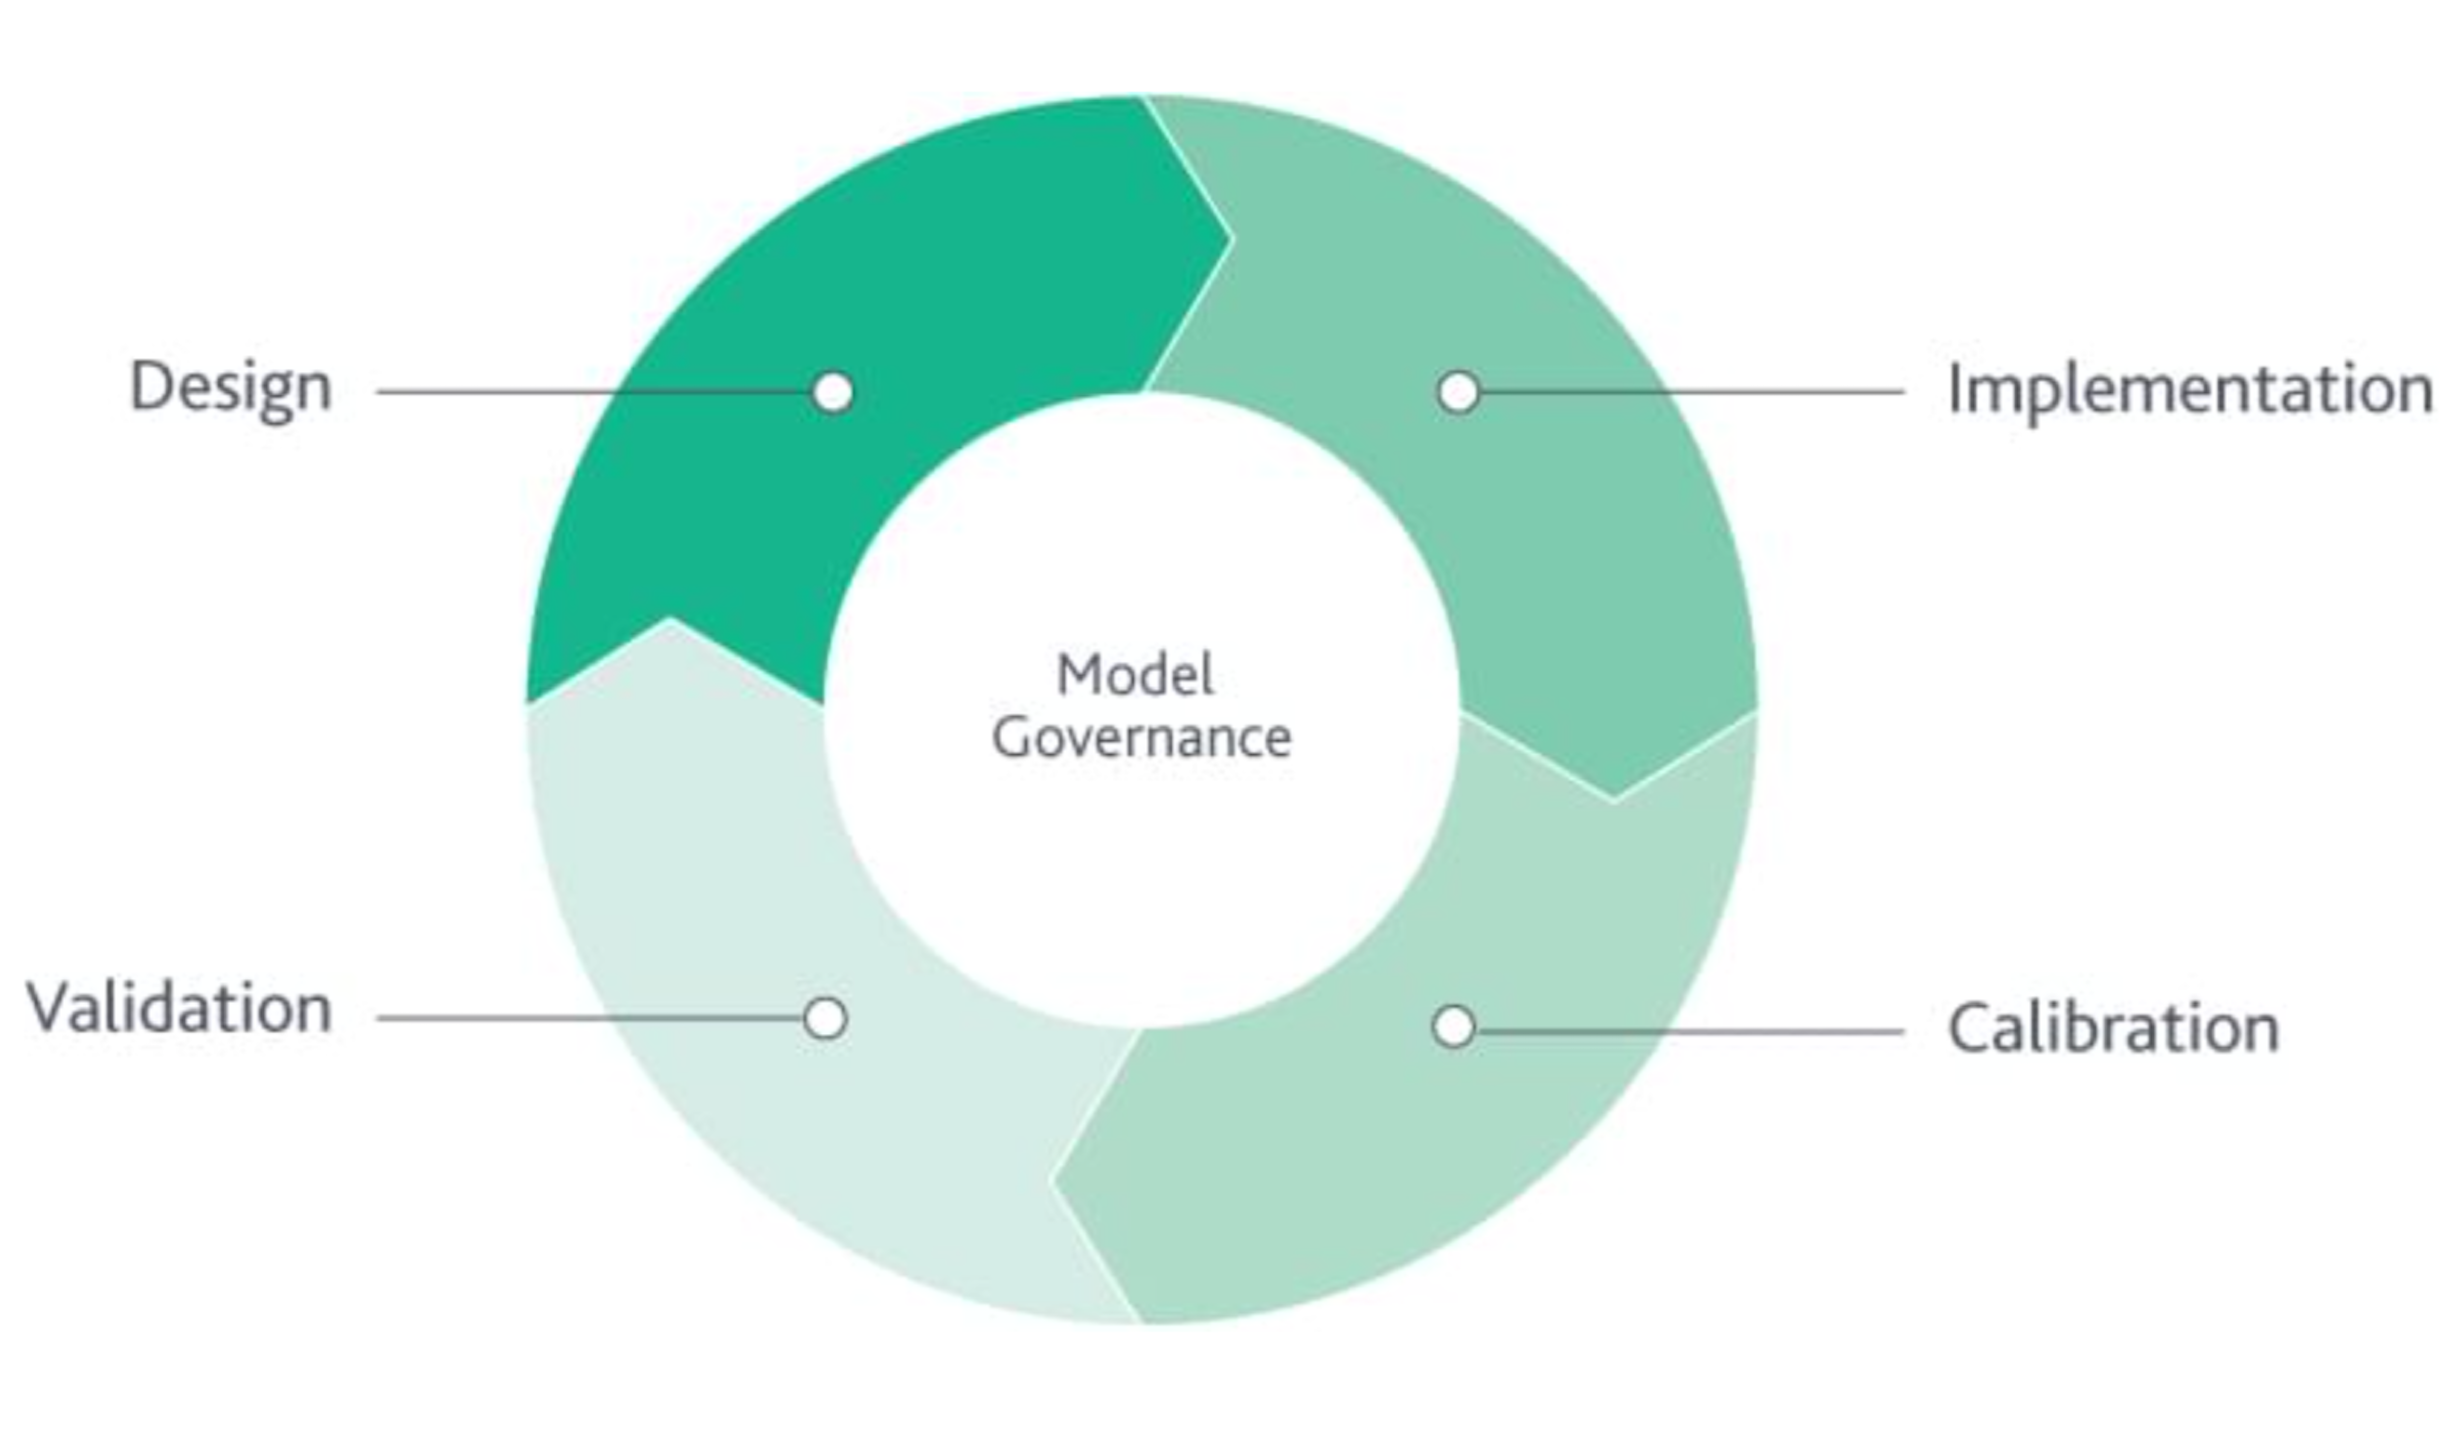
\includegraphics[width=5cm, height=7cm]{images/model_governance_lifecycle2} }}%
%%	\qquad
%%	\subfloat[Development]{{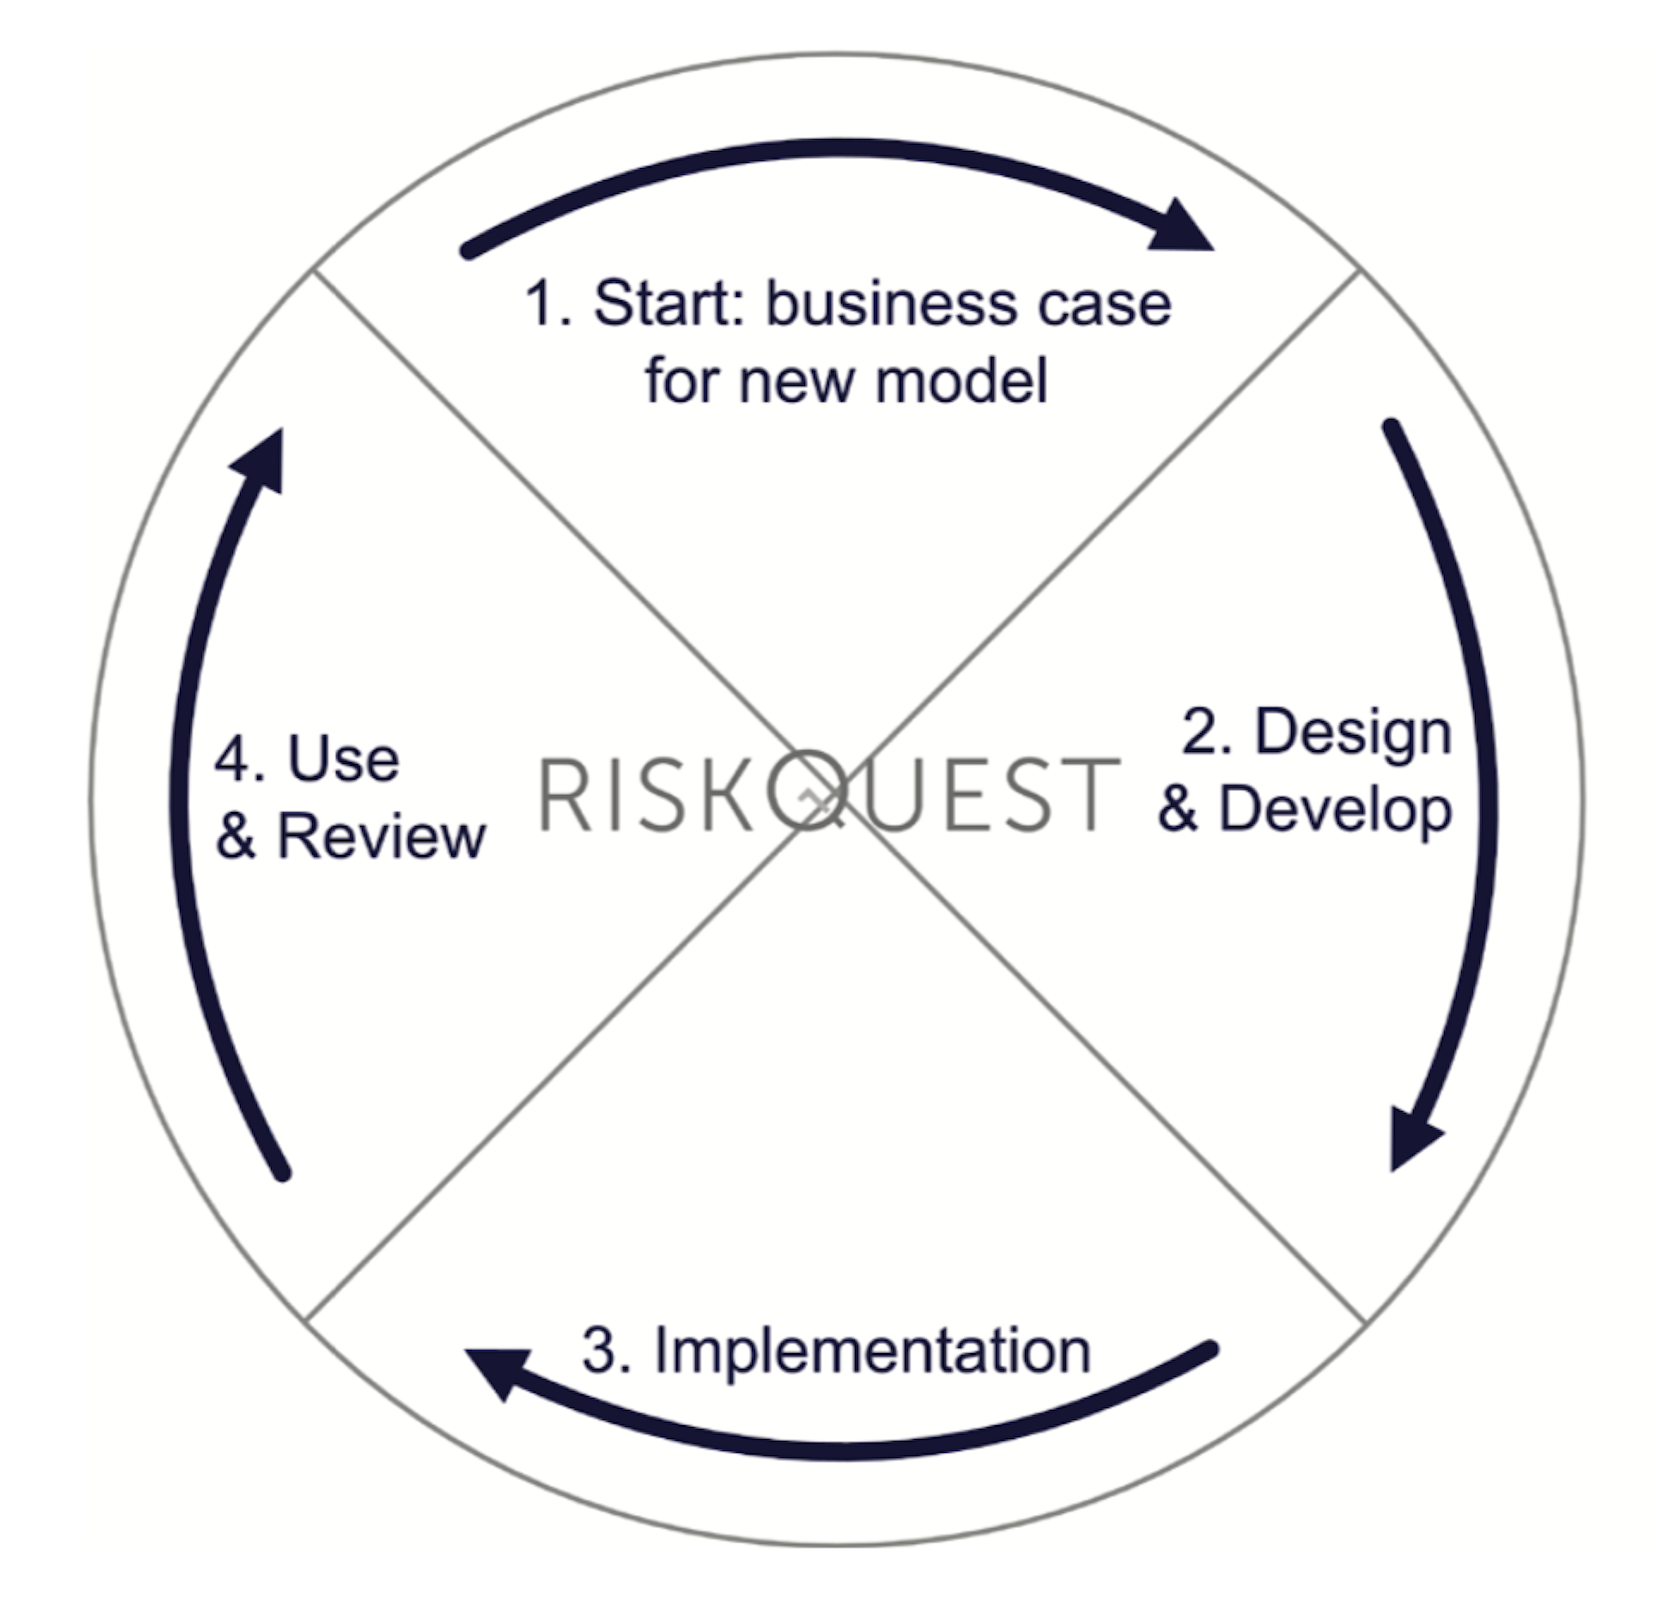
\includegraphics[width=5cm, height=7cm]{images/model_lifecycle2} }}%
%%\end{figure}
%%\end{frame}
%
%\begin{frame}
%\frametitle{Model governance lifecycle}
%Overall governance set around a model’s lifecycle
%\begin{itemize}
%\item model development (design)
%\item model implementation
%\item model calibration
%\item model validation
%\end{itemize} 
%\end{frame}
%
%
%%\begin{frame}
%%\frametitle{8 key elements for a solid model governance framework}
%%\begin{figure}[h]
%%	\centering
%%	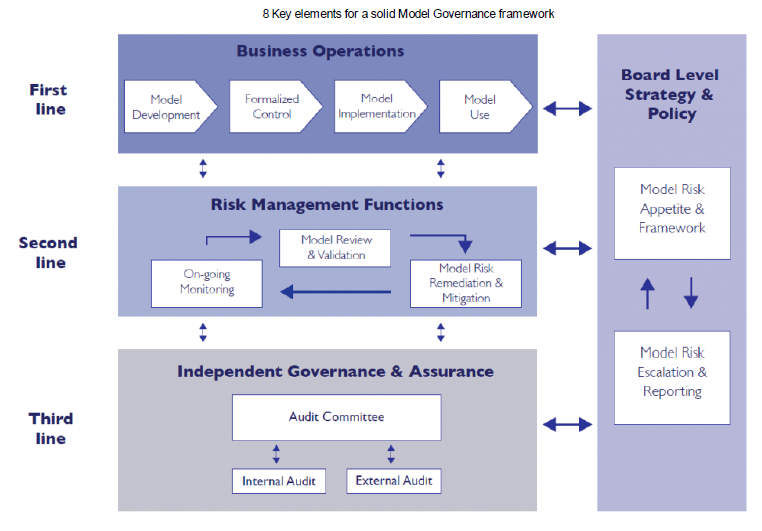
\includegraphics[scale=.5]{images/gov1}
%%\end{figure}
%%\end{frame}
%
%\begin{frame}
%\frametitle{Model governance best practices}
%\begin{itemize}
%	\item model definitions
%	\item model inventory
%	\item model categorization
%	\item model risk teams
%\end{itemize}
%\end{frame}
%
%\begin{frame}
%\frametitle{References}
%\begin{enumerate}
%	\item https://odsc.medium.com/continuous-delivery-for-machine-learning-d07f2d0f051
%\end{enumerate}
%\end{frame}

\end{document}